%\begin{filecontents}{apsrevcontrol.bib}
%  @CONTROL{apsrev41Control,title="0"%,author="48",editor="1",pages="1",year="0"}
%\end{filecontents}
\RequirePackage[l2tabu, orthodox]{nag}
\RequirePackage{fixltx2e}
\RequirePackage{fix-cm}
\PassOptionsToPackage{pdftex,psdextra=true,
pdfversion=1.7,
pdfencoding=auto,
pdfnewwindow=true,
pdfusetitle=true,
psdextra=true,
pdftoolbar=false,
pdfmenubar=false,
bookmarks=true,
bookmarksnumbered=true,
bookmarksopen=true,
pdfpagemode=UseThumbs,
bookmarksopenlevel=1,
pdfpagelabels=false
}{hyperref}
\documentclass[aps,english,superscriptaddress,onecolumn,twoside,longbibliography,pra,floatfix,fleqn,nofootinbib]{revtex4-1}%


\usepackage[utf8]{inputenx}% for arXiv use encoding ansinew
%\input{ix-utf8enc.dfu}
%\usepackage[utf8x]{inputenc}% for arXiv use encoding ansinew
\usepackage[OT1]{fontenc}

\usepackage{amsfonts}
\usepackage{amssymb}
\usepackage{amsthm}
\usepackage[intlimits]{amsmath}
%\usepackage{mathdots}
\usepackage{graphicx}%
\usepackage{placeins} %for FloatBarrier
\usepackage{afterpage} %for FloatBarrier in afterpage wrapper
%\usepackage{flushend}
%\usepackage{dblfloatfix}
\usepackage[normalem]{ulem} %for sout
\usepackage[raggedright,bf,nooneline]{subfigure}
\renewcommand{\thesubfigure}{\alph{subfigure}}
\usepackage{paralist}
%\usepackage{ellipsis}
\usepackage{float}% (not with floatrow)
\usepackage{wrapfig}
%\usepackage{floatrow}

\setcounter{MaxMatrixCols}{30}
\providecommand{\U}[1]{\protect\rule{.1in}{.1in}}
%EndMSIPreambleData
\newtheorem{theorem}{Theorem}
\newtheorem{acknowledgement}[theorem]{Acknowledgement}
\newtheorem{algorithm}[theorem]{Algorithm}
\newtheorem{axiom}[theorem]{Axiom}
\newtheorem{claim}[theorem]{Claim}
\newtheorem{conclusion}[theorem]{Conclusion}
\newtheorem{condition}[theorem]{Condition}
\newtheorem{conjecture}[theorem]{Conjecture}
%\newtheorem{corollary}[theorem]{Corollary}
\newtheorem{corollary}{Corollary}[theorem]
\newtheorem{criterion}[theorem]{Criterion}
\newtheorem{definition}[theorem]{Definition}
\newtheorem{example}[theorem]{Example}
\newtheorem{exercise}[theorem]{Exercise}
\newtheorem{lemma}[theorem]{Lemma}
\newtheorem{notation}[theorem]{Notation}
\newtheorem{problem}[theorem]{Problem}
\newtheorem{prop}{Proposition}
\newtheorem{taut}{Tautology}
\newtheorem{remark}[theorem]{Remark}
\newtheorem{solution}[theorem]{Solution}
\newtheorem{summary}[theorem]{Summary}
%\newenvironment{proof}[1][Proof]{\noindent\textbf{#1.} }{\ \rule{0.5em}{0.5em}}

% hyperlink stuff
\usepackage[usenames,dvipsnames]{xcolor}
\definecolor{ultramarine}{RGB}{63, 0, 255}
\definecolor{medblue}{RGB}{0, 0, 100}
\definecolor{panblue}{RGB}{0,24,150}
\definecolor{carmine}{RGB}{150, 0, 24}
\usepackage[breaklinks=true]{hyperref}
\hypersetup{colorlinks,
linkcolor=carmine,
citecolor=medblue,
urlcolor=panblue,
anchorcolor=OliveGreen}
%\usepackage{url}


\definecolor{purple}{RGB}{128,0,128}
\definecolor{PURPLE}{RGB}{128,0,128}
\definecolor{BLACK}{RGB}{0,0,0}
\definecolor{ultramarine}{RGB}{63, 0, 255}
\definecolor{medblue}{RGB}{0, 0, 100}
\definecolor{panblue}{RGB}{0,24,150}
\definecolor{carmine}{RGB}{150, 0, 24}
\definecolor{gray}{RGB}{150, 150, 150}

\newcommand{\purp}[1]{{\color{purple}{#1}\color{black}}}
\newcommand*{\mred}[1]{{\color{RawSienna}{\mathbf{#1}}}}
\newcommand*{\mblue}[1]{{\color{MidnightBlue}{\ensuremath{#1}}}}
\newcommand*{\mpurp}[1]{{\color{Plum}{\mathbf{#1}}}}
\newcommand*{\mgreen}[1]{{\color{OliveGreen}{\mathbf{#1}}}}
\newcommand*{\tred}[1]{{\color{carmine}{\textbf{#1}}}}
\newcommand*{\tblue}[1]{{\color{MidnightBlue}{\textbf{#1}}}}
\newcommand*{\tpurp}[1]{{\color{Plum}{\textbf{#1}}}}
\newcommand*{\tgreen}[1]{{\color{Sepia}{\textbf{#1}}}}

\newcommand{\quoteby}{\raise.17ex\hbox{$\scriptstyle\sim$}}

\usepackage{verbatim} %for comment command
\usepackage{units}% for nicefrac
\newcommand{\half}[1]{\nicefrac{#1}{2}}

%\usepackage{braket} %provide \bra and \Bra and \set and \Set etc...
%\newcommand{\brackets}[1]{\lbrace{#1\rbrace}}
%\newcommand{\brackets}{\Set}



\usepackage{microtype}
%\usepackage{MnSymbol}
%\usepackage{mathabx}

\usepackage[capitalise]{cleveref}
\Crefname{eqs}{Eqs.}{Eqs.}

\creflabelformat{eqs}{(#2#1#3)}
\crefrangelabelformat{equation}{(#3#1#4-#5#2#6)}
%\crefmultiformat{equation}{eqs.~(#2#1#3)}{ and~(#2#1#3)}{, (#2#1#3)}{ and~(#2#1#3)}
\Crefmultiformat{equation}{Eqs.~(#2#1#3}{,#2#1#3)}{,#2#1#3}{,#2#1#3)}
\crefrangelabelformat{eqs}{(#3#1#4-#5#2#6)}
\Crefmultiformat{eqs}{Eqs.~(#2#1#3}{,#2#1#3)}{,#2#1#3}{,#2#1#3)}
\Crefname{prop}{\textbf{Prop}.}{\textbf{Props}.}
\Crefname{taut}{\textbf{Taut}.}{\textbf{Tauts}.}
\Crefname{section}{Sec.}{Secs.}

%\Crefname{ineq}{Ineq.}{Ineqs.}
%\creflabelformat{ineq}{(#2#1#3)}
%\crefrangelabelformat{ineq}{(#3#1#4-#5#2#6)}
%\Crefmultiformat{ineq}{Ineqs.~(#2#1#3}{,#2#1#3)}{,#2#1#3}{,#2#1#3)}

%\Crefname{ineqs}{Ineqs.}{Ineqs.}
%\creflabelformat{ineqs}{(#2#1#3)}
%\crefrangelabelformat{ineqs}{(#3#1#4-#5#2#6)}
%\Crefmultiformat{ineqs}{Ineqs.~(#2#1#3}{,#2#1#3)}{,#2#1#3}{,#2#1#3)}

\newcounter{step}[section]
\newenvironment{step}[1][]{\refstepcounter{step}\par\medskip
   \noindent \textbf{Step~\thestep}\rmfamily#1}{\par\medskip\par}
%\newenvironment{step}[1][Step]{\noindent\textbf{#1.} }{\ \rule{0.5em}{0.5em}}
\Crefname{step}{Step}{Steps}
\creflabelformat{step}{#2#1#3}
\crefrangelabelformat{step}{#3#1#4-#5#2#6}
\Crefmultiformat{step}{Steps.~#2#1#3}{,#2#1#3}{,#2#1#3}{,#2#1#3}
\renewcommand{\thestep}{\arabic{step}}


\usepackage{mathtools} %for mathclap and prescript and more. Learning to love this package. And DeclarePairDelimeter!
\DeclarePairedDelimiter{\ceil}{\lceil}{\rceil}
\DeclarePairedDelimiter{\floor}{\lfloor}{\rfloor}
\DeclarePairedDelimiter{\parens}{\lparen}{\rparen}
\DeclarePairedDelimiter{\parenths}{\lparen}{\rparen}
\DeclarePairedDelimiter{\abs}{\lvert}{\rvert}
\DeclarePairedDelimiter{\norm}{\lVert}{\rVert}
\DeclarePairedDelimiter{\braces}{\lbrace}{\rbrace}
\DeclarePairedDelimiter{\bracks}{\lbrack}{\rbrack}
\DeclarePairedDelimiter{\expec}{\langle}{\rangle}
\newcommand{\brackets}[1]{\braces*{#1}}

%\usepackage{nath} %automatically pair delimiters. Provides \inline and \displayed. Adjusts \frac and /

\newcommand{\na}{\ensuremath{\mathring{a}}}
\newcommand{\nb}{\ensuremath{\mathring{b}}}
\newcommand{\nc}{\ensuremath{\mathring{c}}}

\newcommand{\naf}{\ensuremath{\lnot a}}
\newcommand{\nbf}{\ensuremath{\lnot b}}
\newcommand{\ncf}{\ensuremath{\lnot c}}

\newcommand{\n}[1]{\ensuremath{\overline{#1}}}
\newcommand{\ot}[1]{\ensuremath{\overline{#1}}}
\newcommand{\Nor}[1]{\operatorname{\mathsf{Nor}}\!\bracks*{#1}}

\newcommand{\larray}[1]{\ensuremath{\begin{array}{l}#1\end{array}}}
\newcommand{\lparens}[1]{\ensuremath{\parens*{\larray{#1}}}}
%\newcommand{\NamedFunction}[2]{\operatorname{\mathsf{#1}}\!\bracks*{#2}}
\newcommand{\NamedFunction}[2]{\operatorname{\mathsf{#1}}\!\bracks*{\larray{#2}}}

\newcommand{\nap}{\ensuremath{a'}}
\newcommand{\nbp}{\ensuremath{b'}}
\newcommand{\ncp}{\ensuremath{c'}}
\newcommand{\napp}{\ensuremath{a''}}
\newcommand{\nbpp}{\ensuremath{b''}}
\newcommand{\ncpp}{\ensuremath{c''}}

\newcommand{\p}[1]{p\parenths{#1}}
\newcommand{\pdf}[1]{\operatorname{\mathsf{PDF}}\!\parenths{#1}}
\newcommand{\cramp}[1]{\ensuremath{\mathord{#1}}}
%\newcommand{\cramp}[1]{\ensuremath{\mathopen{}#1\mathclose{}}} oldway. New way is better.
\newcommand{\eql}{\cramp{=}}

\usepackage{bm}
\newcommand{\setlambda}{\bm{\lambda}}



\let\stdsection\section
%\renewcommand\section{\clearpage\stdsection}%every section new page
\begin{document}
\section{Bell Scenario}
\begin{figure*}[t!]
\centering
\subfigure[\hspace{-0.5ex}:\hspace{1ex} The causal structure of the Bell scenario. Conventionally $S$ and $T$ are considered experimental settings; we depict the \tred{latent completed} structure, in which we imagine the settings are selected according to some local hidden variables.\hfill]
{\begin{minipage}[t]{.45\textwidth}
    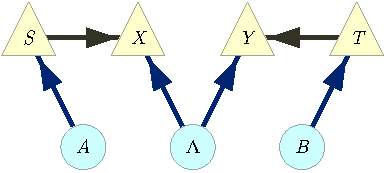
\includegraphics[width=2.55in]{OldFigures/GenuineBellDAG.pdf}
    \label{fig:BellDAG}
\end{minipage}}\hfill{\color{gray}\rule[-0.4cm]{0.5pt}{3cm}}\hfill
\subfigure[\hspace{-0.5ex}:\hspace{1ex} The \tred{latent reduction} of the Bell scenario. Influences between observables have been deleted, but every observable is now directly connected to all of its latent ancestors. See Fig.~1 in Ref. \cite{fritz2012bell}. \hfill]
{\begin{minipage}[t]{.45\textwidth}
    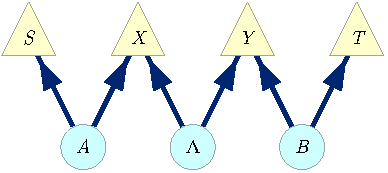
\includegraphics[width=2.55in]{OldFigures/EffectiveBellDAG.pdf}
    \label{fig:EffBellDAG}
\end{minipage}}
\vspace{-2ex}\caption{The Bell scenario: A scenario in which ${X}\cramp{\perp}{T}$ and ${Y}\cramp{\perp}{S}$ but ${X}\cramp{\not\perp}{Y}$. The Bell scenario is particularly famous in quantum theory \cite{bell1966lhvm,Brunner2013Bell,WoodSpekkens}, as many non-local correlations have be generated by replacing $\Lambda$ with some quantum $\bm\rho$.}
\label{fig:Bell}\vspace{-2ex}
\end{figure*}

Consider the causal structure associated to the Bell/CHSH \cite{bell1964einstein,Brunner2013Bell,bell1966lhvm,CHSHOriginal} experiment [\citealp{pusey2014gdag}~(Fig.~E\#2), \citealp{WoodSpekkens}~(Fig.~19), \citealp{chaves2014novel}~(Fig.~1), \citealp{BeyondBellII}~(Fig.~1), \citealp{wolfe2015nonconvexity}~(Fig.~2b), \citealp{steeg2011relaxation}~(Fig.~2)], depicted here in \cref{fig:BellDAG}. $\brackets{S,T,X,Y}$ are all observable variables and $\Lambda$ is the latent common cause of $X$ and $Y$.

%Without loss of generality let's assume that the values $\Lambda\mathopen{=}\lambda$ are drawn from some (possibly infinite, possibly continuous) set $\lambda\in\Omega$. 
The assumption of causal structure dictates that
\begin{align}\begin{split}\label{eq:bellstructure}
%\p{x y s t | \lambda a b}=\p{x_{\lambda a} y_{\lambda b} s_x t_y}
\p{x_{\lambda a b}}=\p{x_{\lambda a}} \,,\; \p{y_{\lambda a b}}=\p{y_{\lambda b}} \,,\; \p{s_{\lambda a b}}=\p{s_{a}} \,,\; \p{t_{\lambda a b}}=\p{t_{b}} \,,%\quad\text{and hence}\quad \p{x y s t | \lambda a b}=\p{x_{\lambda a} y_{\lambda b} s_x t_y}\,,
%=\p{x_{s|\lambda}}\p{y_{t|\lambda}}
\end{split}\end{align}
and hence
\begin{align}\begin{split}\label{eq:bellintegration}
&\p{x y s t | \lambda a b}=\p{x_{\lambda a} y_{\lambda b} s_a t_b}\,,\quad\text{and accordingly}\quad \p{x y s t}=\sum\limits_{{\lambda\in \norm{\Lambda}}}\sum\limits_{{a\in \norm{A}}}\sum\limits_{{b\in \norm{B}}}\p{x_{\lambda a} y_{\lambda b} s_a t_b}\p{\lambda}\p{a}\p{b}.
\end{split}\end{align}
These ancestral-latent dependencies per \cref{eq:bellstructure} are used to map the genuine Bell causal structure (\cref{fig:BellDAG}) to its latent reduction, namely \cref{fig:EffBellDAG}, which \tred{implies the same latent independencies}. The Bell causal structure is known to be lossless under latent reduction \citep[Thm.~2.4]{fritz2012bell}, so \cref{fig:BellDAG} and \cref{fig:EffBellDAG} are indeed observationally equivalent.

An important causal criterion is as follows. 
\begin{prop} \label{prop:CH}
The Bell causal structure (\cref{fig:Bell}) implies that
\begin{align*}
\p{x^1 y^1 s^1 t^1} \p{x^2 y^2 s^2 t^2}
\leq
\p{x^2 s^2 t^1} \p{x^1 y^3 s^1 t^2}
+\p{y^2 s^1 t^2} \p{x^3 y^1 s^2 t^1}
+\p{s^1 t^1} \p{\n{x^3} \n{y^3} s^2 t^2}
\end{align*}
\end{prop}

\begin{proof}
To prove \cref{prop:CH}, start with this logical tautology pursuant to \cref{fig:EffBellDAG}
\begin{align}\begin{split}
\NamedFunction{And}{ x^1_{\lambda ^1 a^1} , y^1_{\lambda ^1 b^1} , s^1_{a^1} , t^1_{b^1} , x^2_{\lambda ^2 a^2} , y^2_{\lambda ^2 b^2} , s^2_{a^2} , t^2_{b^2} }
\implies 
\NamedFunction{Or}{
    \NamedFunction{And}{ x^2_{\lambda ^2 a^2} , s^2_{a^2} , t^1_{b^1} , x^1_{\lambda ^1 a^1} , y^3_{\lambda ^1 b^2} , s^1_{a^1} , t^2_{b^2} } ,\\
    \NamedFunction{And}{ y^2_{\lambda ^2 b^2} , s^1_{a^1} , t^2_{b^2} , x^3_{\lambda ^1 a^2} , y^1_{\lambda ^1 b^1} , s^2_{a^2} , t^1_{b^1} } ,\\
    \NamedFunction{And}{ s^1_{a^1} , t^1_{b^1} , \n{x^3_{\lambda ^1 a^2}} , \n{y^3_{\lambda ^1 b^2}} , s^2_{a^2} , t^2_{b^2} } 
}
\end{split}\end{align}
which converts to the inequality
\begin{align}\begin{split}\label{eq:bellstructineq}
\p{x^1_{\lambda ^1 a^1} y^1_{\lambda ^1 b^1} s^1_{a^1} t^1_{b^1}} \p{x^2_{\lambda ^2 a^2} y^2_{\lambda ^2 b^2} s^2_{a^2} t^2_{b^2}}
\leq
\lparens{
\hphantom{+}\p{x^2_{\lambda ^2 a^2} s^2_{a^2} t^1_{b^1}} \p{x^1_{\lambda ^1 a^1} y^3_{\lambda ^1 b^2} s^1_{a^1} t^2_{b^2}}
\\+\p{y^2_{\lambda ^2 b^2} s^1_{a^1} t^2_{b^2}} \p{x^3_{\lambda ^1 a^2} y^1_{\lambda ^1 b^1} s^2_{a^2} t^1_{b^1}}
\\+\p{s^1_{a^1} t^1_{b^1}} \p{\n{x^3_{\lambda ^1 a^2}} \n{y^3_{\lambda ^1 b^2}} s^2_{a^2} t^2_{b^2}}
}
\end{split}\end{align}
or, equivalently,
\begin{align}
\p{x^1 y^1 s^1 t^1|\lambda ^1 a^1 b^1} \p{x^2 y^2 s^2 t^2|\lambda ^2 a^2 b^2}
\leq
\lparens{
\hphantom{+}\p{x^2 s^2 t^1|\lambda ^2 a^2 b^1} \p{x^1 y^3 s^1 t^2|\lambda ^1 a^1 b^2}
\\+\p{y^2 s^1 t^2|\lambda ^2 b^2 a^1} \p{x^3 y^1 s^2 t^1|\lambda ^1 a^2 b^1}
\\+\p{s^1 t^1|a^1 b^1} \p{\n{x^3} \n{y^3} s^2 t^2|\lambda ^1 a^2 b^2}
}\,.
\end{align}
To complete the proof we simply marginalize both sides over $\brackets{\lambda ^1, a^1, b^1,\lambda ^2, a^2, b^2}$.\end{proof}


A special case of \cref{prop:CH} is obtained by setting $\brackets{x^2,y^2}\to\mathsf{True}$, $x^3\to \n{x^1}$, and $y^3\to \n{y^1}$. This yields
\begin{align}
\p{x y s^1 t^1} \p{s^2 t^2}
\leq
\p{s^2 t^1} \p{x \n{y} s^1 t^2}
+\p{s^1 t^2} \p{\n{x} y s^2 t^1}
+\p{s^1 t^1} \p{x y s^2 t^2}
\end{align}
which is better understood in conditional form, namely
\begin{align}
\p{x y | s^1 t^1} \p{s^1 t^1}\p{s^2 t^2}
\leq
\p{x \n{y} | s^1 t^2}\p{s^1 t^2}\p{s^2 t^1} 
+\p{\n{x} y | s^2 t^1}\p{s^2 t^1}\p{s^1 t^2} 
+\p{x y | s^2 t^2}\p{s^2 t^2}\p{s^1 t^1}.
\end{align}
However, the Bell scenario causal structure further implies that $\p{s t}=\p{s}\p{t}$, and hence
\begin{align}
\p{x y | s^1 t^1}
\leq
\p{x \n{y} | s^1 t^2}
+\p{\n{x} y | s^2 t^1}
+\p{x y | s^2 t^2}.
\end{align}
Finally, we may eliminate negation notation entirely by substituting $\p{x \n{y} | s t} \to \p{x | s t}-\p{x y | s t} = \p{x | s}-\p{x y | s t}$ etc. Thus we obtain
\begin{align}
\p{x y | s^1 t^1} + \p{x y | s^1 t^2} + \p{x y | s^2 t^1}
\leq
\p{x | s^1}
+\p{y | t^1}
+\p{x y | s^2 t^2}.
\end{align}
which is simply the Clauser-Horne (CH) inequality \cite{CHInequality} for the Bell scenario. The CH inequality is the \emph{unique} Bell inequality (up to permutations) for the Bell scenario if $\brackets{S,T,X,Y}$ are all binary, and hence the CH inequality is a necessary and sufficient criterion to ascertain if correlations are compatible with that Bell scenario variant.

\setlength{\bibsep}{3pt plus 3pt minus 2pt}
\bibliographystyle{apsrev4-1}
\nocite{apsrev41Control}
\bibliography{apsrevcontrol,hardyinference}
\end{document}